SmartOrder \`e una web application: per accedervi \`e sufficiente aprire il browser\textsubscript{\textit{g}} e navigare all'indirizzo fornito dall'azienda. Non \`e richiesta alcuna installazione.

\subsection{Schermata di login}

\begin{figure}[H]
    \centering
    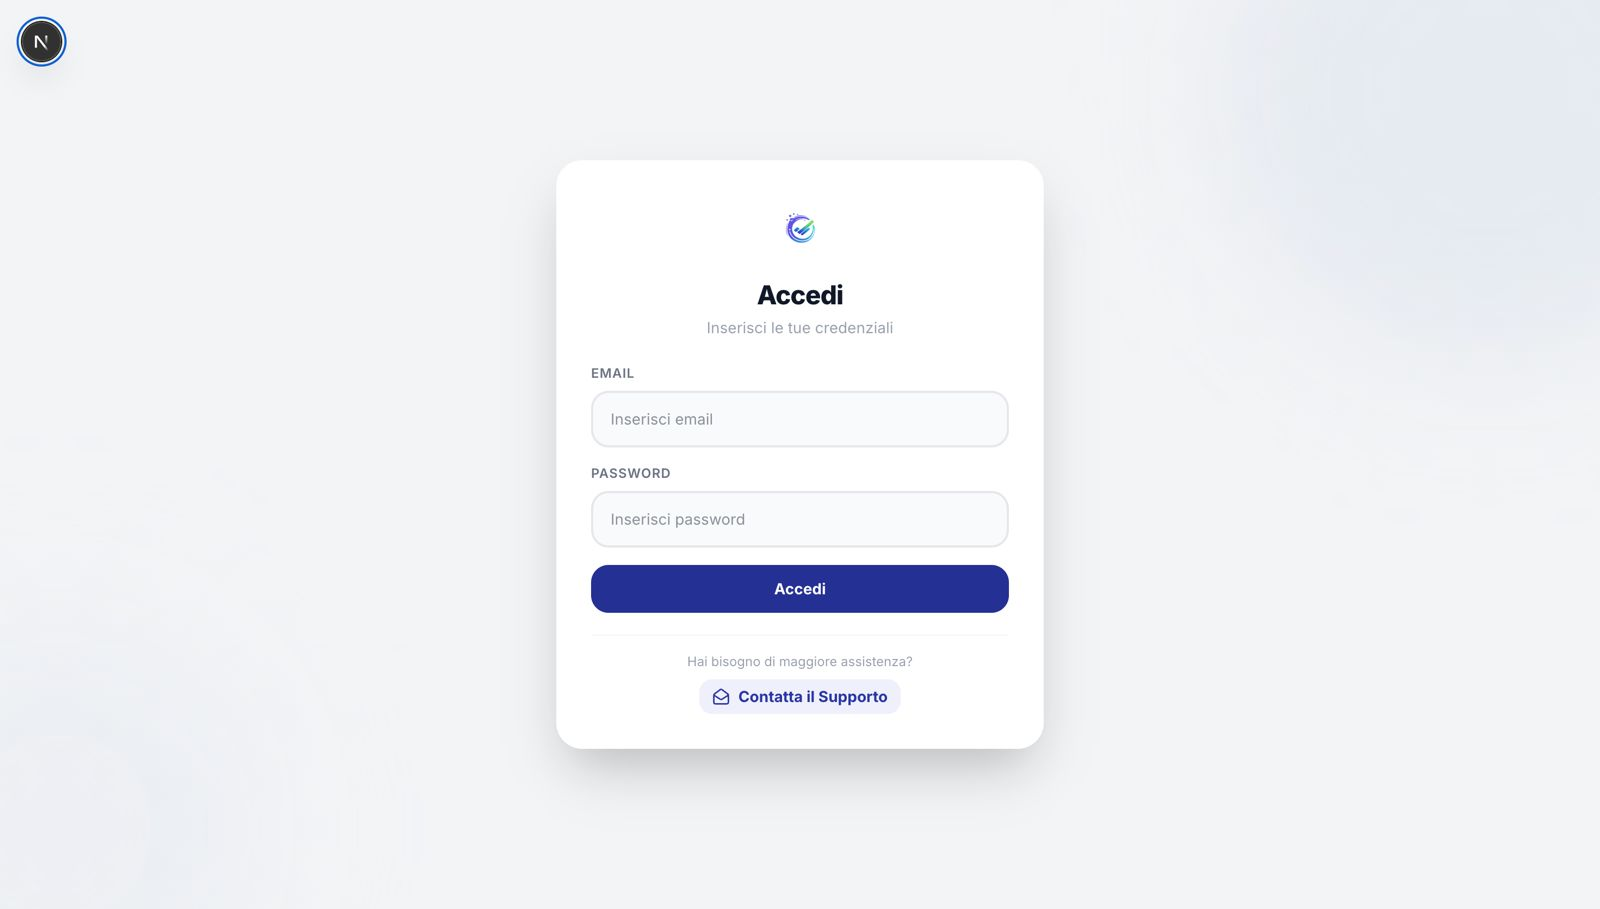
\includegraphics[width=0.7\textwidth]{Contenuti/immagini/login.jpeg}
    \caption{Schermata di login}
\end{figure}

All'apertura dell'applicazione viene visualizzata la schermata di autenticazione. L'utente inserisce le proprie credenziali (email e password) fornite dall'azienda nei campi dedicati e preme il pulsante \textbf{Accedi}.

Se le credenziali sono corrette e l'utente ha ruolo \textbf{Cliente}, viene immediatamente reindirizzato all'interfaccia principale di ordinazione. Se le credenziali appartengono a un utente con ruolo \textbf{Operatore}, viene effettuato un redirect automatico all'interfaccia di backoffice.

\`E inoltre possibile contattare il supporto direttamente dalla schermata di login tramite il pulsante \textbf{Contatta il Supporto}, che apre il client di posta predefinito con un template di richiesta assistenza precompilato.

\subsection{Logout}
Per disconnettersi dalla piattaforma, selezionare l'opzione \textbf{Logout} dal menu dell'area personale. La sessione viene invalidata e l'utente viene riportato alla schermata di login.
